\section{Estensione del Modello}
In questa sezione verrano descritte le modifiche e le aggiunte effettuate al modello base,
% TODO: riscrivere
ma prima verrano evidenziate le limitazioni e le mancanze del modello anche rispetto allo stato dell'arte.

Molte assunzioni sono poco realistiche come la velocità costante dei pedoni, tutte le strade a senso unico e l'assenza di interazioni nelle
intersezioni.
%
Inoltre viene assunto che tutti gli agenti conoscano il percorso più breve per il rifugio.
%
Un'altra limitazione riguarda le interazioni tra i vari tipi di agenti.
Questo modello considera esclusivamente le interazioni auto-auto
tramite il modello General Motors, ma non prevede nessuna interazione pedone-pedone o pedone-auto.

% TODO: riscrivere
Come è stato appena descritto le interazioni tra gli agenti
hanno un ampio margine per essere ?rappresentate?, in particolare ci si concentrerà sulle interazioni nelle intersezioni
introducendo meccanismi di coordinazione tra i vari tipi di agente. Inoltre la velocità dei pedoni verrà modificata in base alla congestione
in modo da poter rappresentare uno scenario più realistico.

\subsection{Rete Stradale}
Prima di descrivere le varie aggiunte in questa sezione verrannò elencate le varie modifiche che sono state effettuate alla rete stradale.

Tutte le strade della rete sono state considerate come strade locali secondo il \textcite{seaside2010tsp},
ovvero strade a doppio senso e a una corsia con una larghezza variabile da 7.3 m a 9 m e opzionalmente
un marciapiedie per ogni lato della strada con una larghezza fissa di 1.5 m.
%
È stato assunto che tutte le strade abbiano marciapiedi su entrambi i lati e che la larghezza sia fissata al valore minimo.

% TODO: espandere
Sono stati associati gli stop alle strade collegate ad un intersezioni.

\subsection{Speed Variability dei Pedoni}
Riassunto stato dell'arte per la speed variability e survey di modelli macroscopici sui diagrammi fondamentali.

È stata introdotta una variabilità nella velocità di camminata per i pedoni utilizzando il modello di Weiddman con una \textit{free flow speed} di 1.34 m/s
e una \textit{jam density} di 5.4 p/m².
Il calcolo della densità è stato effettuato considerando un'area di ricerca di 4 m x 1.5 m di fronte al pedone,
come in \textcite{goto2012tsunami, wang2021novel}.

I pedoni nel caso in cui sono presenti anche auto, procedono esclusivamente sui marciapiedi, altrimenti occupano tutta la strada.

Spiegare modello di weidmann.

\newpage

\subsection{Gestione degli Intersezioni}
Per la gestione delle intersezioni sono stati considerati esclusivamente gli incroci a 4 strade e trattati come intersezioni di tipo AWSC (All Way Stop Controlled) o TWSC (Two Way Stop controlled).

% TODO: riscrivere, un po' confuso
Tramite l'utilizzo di OpenStreetMap e GoogleMaps, sono state estratte manualmente le informazioni circa la posizione e nel case dei TWSC la direzione
di precedenza di tali tipi di incroci per la citta di Seaside, ottenendo la seguente (Fig. \ref{fig:intersections}).

\begin{figure}[ht]
    \centering
    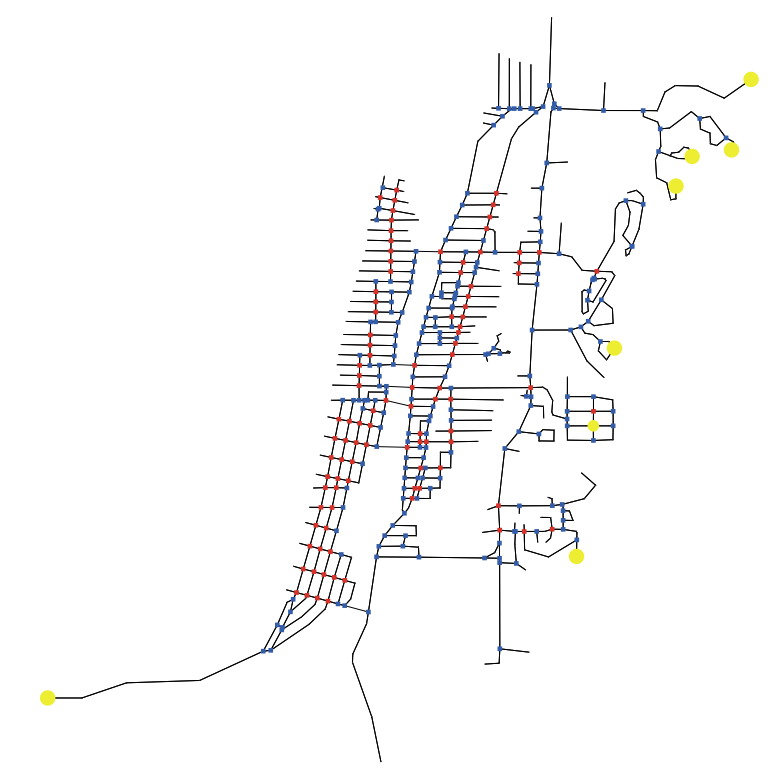
\includegraphics[width=0.7\textwidth]{images/intersections}
    \caption{intersezioni classificate per numero di strade: rosse a 4 strade (98 nodi) e blu a 3 strade (206 nodi).}
    \label{fig:intersections}
\end{figure}

Inoltre nelle intersezioni è stata introdotta una zona di attraversamento per la gestione delle interazioni tra auto e pedoni.
È stato assunto che gli incroci abbiano lunghezza e larghezza pari alla larghezza della strada (10.3 m).
Dal momento che la rappresentazione della strada è network-based è stato deciso che 
la zona iniza prima dell'incrocio e finisce dopo dell'incrocio a una distanza pari alla metà della larghezza (5.15 m) (Fig. \ref{fig:crossing-area}).

\begin{figure}[ht]
    \centering
    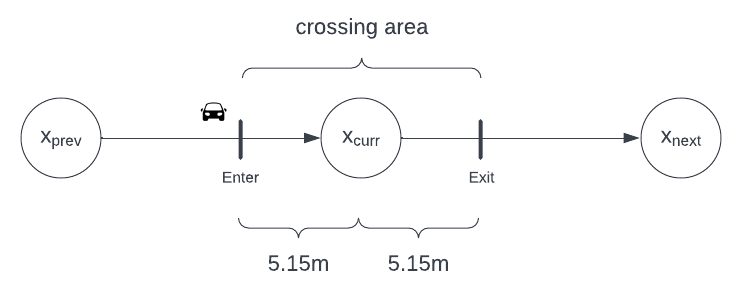
\includegraphics[width=0.5\textwidth]{images/crossing_area}
    \caption{Zona di attraversamento di un'intersezione.}    
    \label{fig:crossing-area}
\end{figure}

\newpage
Per rappresentare l'attraversamento dei pedoni e delle auto sono state aggiunte le seguenti informazioni ad ogni intersezione a 4 strade $i$:
\begin{itemize}
    \item $C_{i, j}$ = numero di pedoni che stanno usando l'attraversamento pedonale che si trova sulla strada che va dall'incrocio $i$ all'incrocio $j$.
    \item $\textit{Arrival}_i$ = coda delle auto nella zona di attraversamento ordinate per tempo di arrivo.
    \item $\textit{Crossing}_i$ = insieme delle auto che possono passare contemporaneamente.
    \item $\textit{Stops}_i$ = insieme delle intersezioni $j$ collegate a $i$ in cui è presente uno stop nella strada $(i, j)$.
\end{itemize}

% Inoltre per i TWSC nelle intersezioni la presenza degli stop viene segnata, mediante una lista con il numero dell'intersezioni interessate.

Per stabilire la posizione all'interno della rete stradale, le precedenze e la direzione della prossima intersezione per ogni agente $x$ 
vengono definite:
\begin{itemize}
    \item $x_{prev}$ l'intersezione precendente
    \item $x_{curr}$ l'intersezione corrente
    \item $x_{next}$ la prossima intersezione
    \item magari anche $x_{side}, x_{dir}$, ...
\end{itemize}

\subsubsection*{Pedoni}
% Dato un pedone $x$ si definiscono $x_{prev}$ l'intersezione precendente, $x_{curr}$ l'intersezione corrente e $x_{next}$ la prossima intersezione.

Data la tripla ($x_{prev}$, $x_{curr}$, $x_{next}$) viene associata ad ogni intersezione collegata a $x_{curr}$ la direzione per raggiungerla seguendo il senso orario a partire da $x_{prev}$,
per cui $I_d$ indica l'intersezione nella direzione $d \in \{\textit{origin}, \textit{left}, \textit{straight}, \textit{right}\}$.
%
La direzione associata all'intersezione $x_{next}$ è quella dove è diretto il pedone e viene identificata da $x_{dir}$.

Quando un pedone $x$ entra nella zona di attraversamento di $x_{curr}$ dall'intersezione $x_{prev}$ e si trova sul marciapiede $x_{side} \in \{ \textit{left}, \textit{right} \}$ 
ha tre direzioni in cui poter andare: \textit{left}, \textit{straight}, \textit{right} (Fig. \ref{fig:pedestria-crossing}):
\begin{itemize}
    \item Se $x_{dir} = \textit{straight}$ e $x_{side} = \textit{side}$ viene incrementato $C_{x_{curr}, I_{\textit{side}}}$ di 1.
    \item Se $x_{dir} = \textit{side}$ e $x_{side} \neq \textit{side}$ viene incrementato $C_{x_{curr}, I_{\textit{origin}}}$ di 1.
    \item Se  $x_{dir} = \textit{side}$ e $x_{side} = \textit{side}$ non viene alterato nessun contatore.
\end{itemize}

Quando il pedone finisce di attraversare il contatore corrispondente viene decrementato di 1.


\begin{figure}[ht]
    \centering
    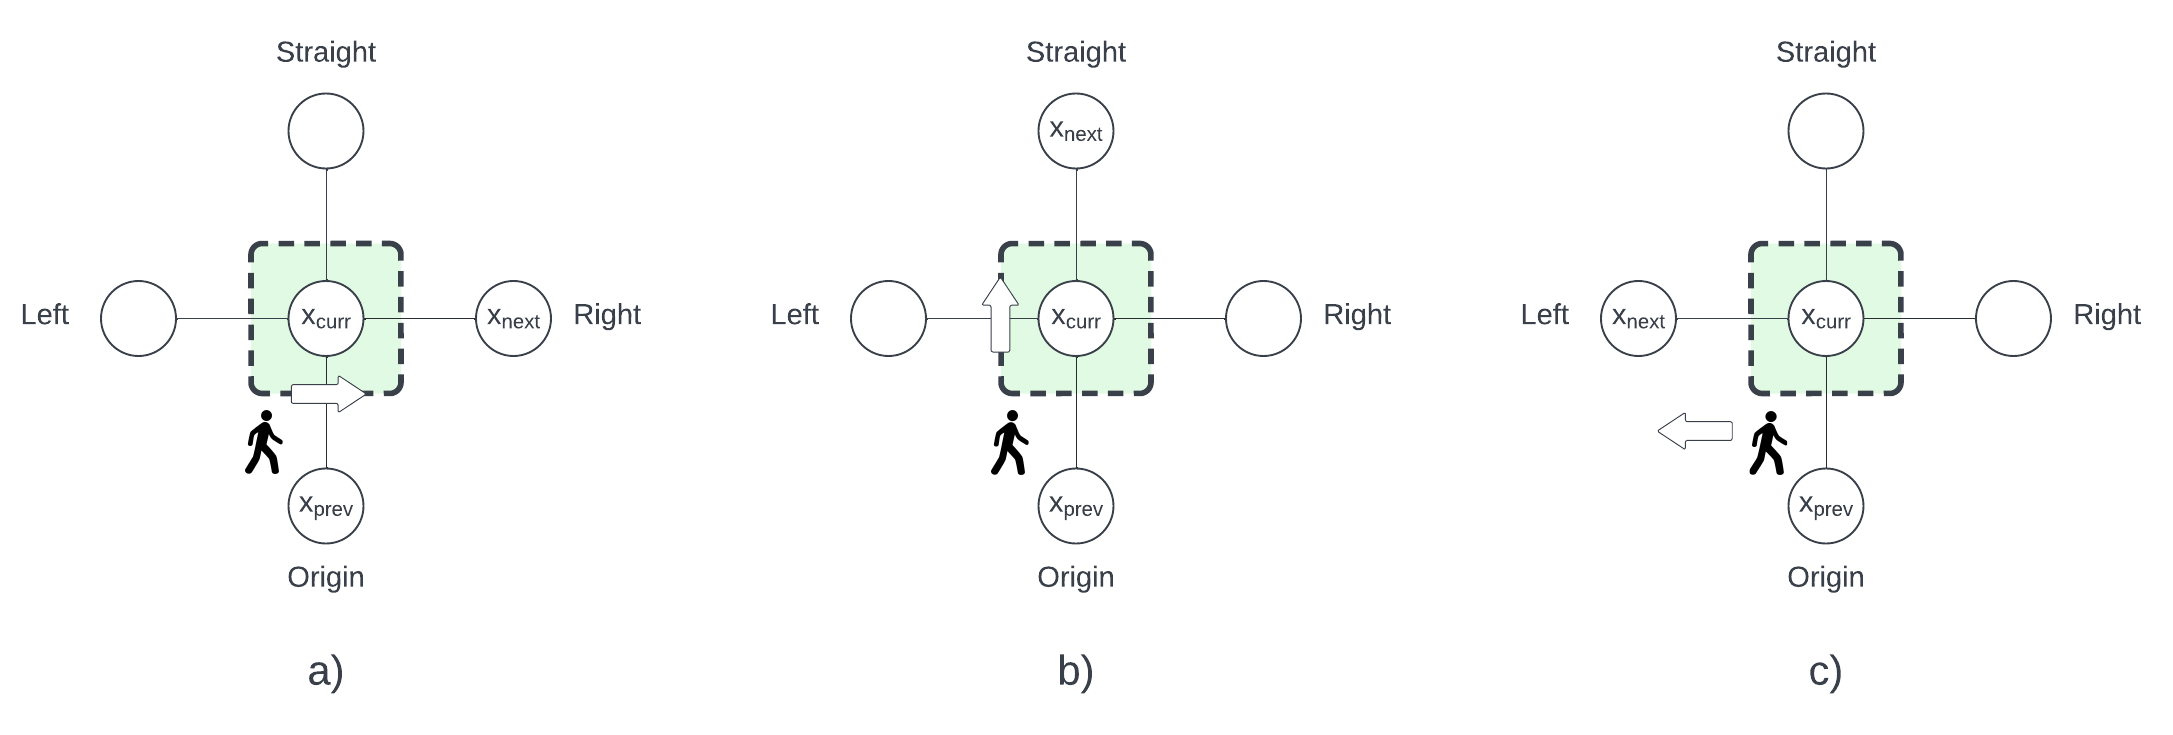
\includegraphics[width=\textwidth]{images/pedestrian_crossing}
    \caption{
        Esempio dei tre casi di attraversamento dal punto di vista del pedone che si trova sul marciapiede sinistro.
        a) il pedone si trova sul lato sinistro e attraversa sul link collegato a origin.
        b) il pedone attraverso sul lato sinistro dell'incrocio, quindi sul link collegato a left.
        c) il pedone segue il marciapiede sulla sinistra senza attraversare.
    }
    \label{fig:pedestria-crossing}
\end{figure}


\subsubsection*{Auto}

La schedulazione e la gestione delle precedenze tra auto verrà descritta successivamente,
mentre qui verrà presentato il funzionamento generale della gestione di un incrocio cosi come già visto per i pedoni.

Le auto quando raggiungono la zona di attraversamento vengono aggiunte alla coda $\textit{Arrival}_i$ e schedulate
in base al tipo d'intersezione (AWSC, TWSC), una volta avuto il via libera le auto sono aggiunte alla coda $\textit{Crossing}_i$.
%
Una volta lasciato l'incrocio vengono rimosse dalle code.

Inoltre, data un auto x che entra nella zona di attraversamento di $x_{curr}$ dall'intersezione $x_{prev}$,
l'agente deve dare la precedenza a possibili pedoni, nello specifico potrà passare se e solo se $C_{x_{curr},x_{prev}}$ = 0 e $C_{x_{curr},x_{next}}$ = 0
\begin{figure}[ht]
    \centering
    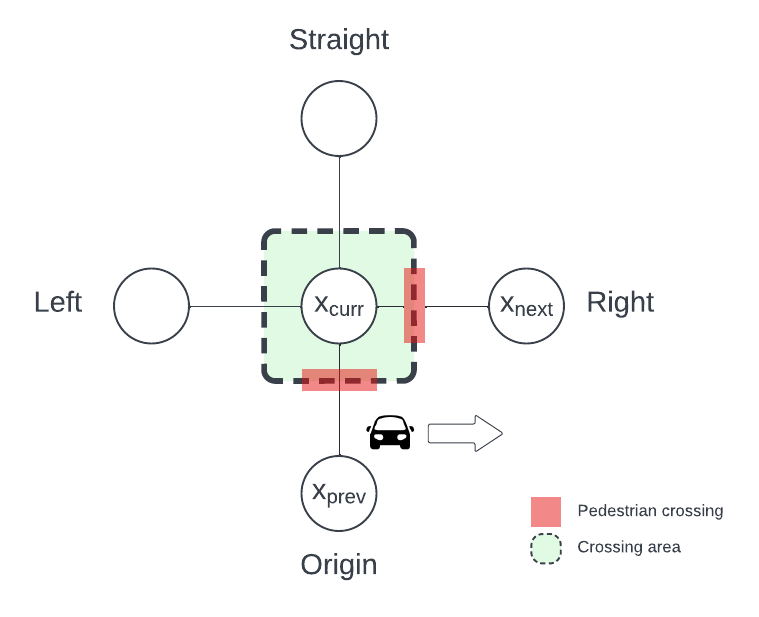
\includegraphics[width=0.45\textwidth]{images/crossing_auto_ped_crossing}
\end{figure}


\newpage



\subsubsection*{Precedenze}
In questa sotto sezione verrano presentate le casistiche in cui hanno il via libera oppure si presentano dei conflitti tra 2 o 3 auto contemporaneamente ad un incrocio.
Inoltre in questo lavoro è stata esclusa la possibilità che 4 auto arrivino contemporaneamente allo stesso incrocio nello stesso momento.

La risoluzione delle precedenze avviene tra le auto che arrivano ad un'intersezione allo stesso tempo. 
L'auto che ha la destra libera viene considerata provenire da \textit{origin} e dal suo punto di riferimento
vengono identificate le direzioni di provenienza delle altre auto. 

Nel caso in cui l'intersezione è di tipo TWSC viene scelta casualmente come riferimento una delle due auto che si trovano 
sulla via principale. Nello stesso modo una volta che la via principale è libera viene gestita l'interazione tra le due auto con stop.

Nelle seguenti tabelle (Tab. \ref{tab:Origin-Left}, Tab. \ref{Origin-Straight}) sono riportati i casi in cui tutte le auto possono passare contemporaneamente o meno.
La risoluzione avviene dall'auto più a destra, che può passare sicuramente, in senso orario. 
Se anche la seconda può passare allora si passa alla terza REF.

\begin{table}[ht]
    \centering
    \begin{tabular}{|c|c|c|c|}
        \hline
        \textbf{Origin-Left} & \textbf{Left} & \textbf{Right} & \textbf{Straight} \\ \hline
        \textbf{Left}        & 0             & 1              & 0                 \\ \hline
        \textbf{Right}       & 1             & 1              & 0                 \\ \hline
        \textbf{Straight}    & 0             & 1              & 0                 \\ \hline
    \end{tabular}
    \caption{Tabella che mostra per il caso Origin-Left le casistiche di conflitto in base a tutte le possibili direzioni prese dalle auto all'incrocio, i casi in cui le auto possono passare contemporaneamente sono segnati con valore 1, 0 altrimenti.
    }
    \label{tab:Origin-Left}
\end{table}


\begin{table}[ht]
    \centering
    \begin{tabular}{|c|c|c|c|}
        \hline
        \textbf{Origin-Straight} & \textbf{Left} & \textbf{Right} & \textbf{Straight} \\ \hline
        \textbf{Left}            & 1             & 0              & 0                 \\ \hline
        \textbf{Right}           & 0             & 1              & 1                 \\ \hline
        \textbf{Straight}        & 0             & 1              & 1                 \\ \hline
    \end{tabular}
    \caption{Tabella che mostra per il caso Origin-Straight le casistiche di conflitto in base a tutte le possibili direzioni prese dalle auto all'incrocio, i casi in cui le auto possono passare contemporaneamente sono segnati con valore 1, 0 altrimenti.}
    \label{Origin-Straight}
\end{table}


Per il confronto a tre Origin-Left-Straight soltanto le casistiche
che permettono il passaggio contemporaneo di tutte le auto verrannò elencate:

\begin{itemize}
    \item Origin-Left-Straight: Right, Left, Right
    \item Origin-Left-Straight: Left, Right, Left
    \item Origin-Left-Straight: Right, Right, Right
    \item Origin-Left-Straight: Straight, Right, Right
\end{itemize}



